% !TEX root = ../lab2_report.tex
% ═══════════════════════════════════════════════════════════════
% 实验六：平面叶栅尾迹损失实验
% ═══════════════════════════════════════════════════════════════

\section{实验六：平面叶栅尾迹损失实验}

\subsection{实验目的}

\begin{enumerate}
    \item 认识叶栅尾迹损失的形成机制和物理机理。
    \item 了解三孔探针尾迹速度分布测量的原理及坐标架操作方法。
    \item 掌握尾迹区气动参数的测量方法和数据处理方法。
    \item 理解边界层理论在叶栅尾迹损失分析中的应用。
\end{enumerate}

\subsection{实验原理}

当气流流经叶栅通道时，叶片表面附面层内因流体黏性耗散造成动量损失。在叶片尾缘，吸力面和压力面的两股附面层汇合脱体，形成一个低总压、低速度的狭长区域——尾迹。尾迹内外的速度差导致湍流掺混，将主流的部分动能不可逆地转化为热能，构成叶型损失的重要组成部分。

本实验在固定攻角（$0\textdegree$）下，利用三孔探针沿叶栅出口截面（周向/栅距方向）逐点扫描，测量尾迹区内的总压和速度分布，分析尾迹的速度亏损特征和尾迹宽度，从而理解尾迹损失的物理机制。

\subsection{实验装置}

\begin{itemize}
    \item 平面叶栅风洞（NACA-65叶型，参数同实验四）
    \item 三孔气动探针及三自由度位移机构
    \item 压力采集系统
    \item 探针转台（用于对向测量）
\end{itemize}

\subsection{实验步骤}

\begin{enumerate}
    \item 将叶栅攻角调至 $0\textdegree$（转盘刻度 $10.6\textdegree$），调节导轨1至刻度 2 cm。
    \item 调节导轨2（周向/栅距方向），将探针移至第3或第4个叶片尾缘左侧的起始位置。
    \item 在每个测量位置，转动探针转台使孔1、孔3压力相等（对向测量），记录中间孔2的读数（当地总压 $P_2^*$）。
    \item 沿导轨2方向以固定步长逐步移动探针，每个位置重复步骤\textbf{3}。
    \item 扫描范围覆盖至少 2 个栅距（约 65 mm），以获取包含至少两个完整尾迹形态的周期性速度分布。
    \item 实验结束：关闭风机，整理设备。
\end{enumerate}

\subsection{数据处理方法}

\subsubsection{速度计算（不可压缩伯努利方程）}

\begin{equation}
    v = \sqrt{\frac{2(P_2^* - P_2)}{\rho}}
\end{equation}

\begin{equation}
    \rho = \frac{P_{\text{atm}}}{R \cdot T_{\text{atm}}}, \quad R = 287.058\ \text{J/(kg·K)}
\end{equation}

式中 $P_2^*$ 为探针测得的当地总压，$P_2$ 为出口截面静压。

\subsubsection{无量纲速度亏损}

以主流区最大速度 $v_{\max}$ 进行无量纲化：
\begin{equation}
    \bar{v} = \frac{v}{v_{\max}}
\end{equation}

尾迹区对应 $\bar{v} < 1$，尾迹中心对应最小 $\bar{v}$ 值。

\subsection{数据处理结果及分析}

\subsubsection{尾迹速度分布}

\begin{figure}[H]
    \centering
    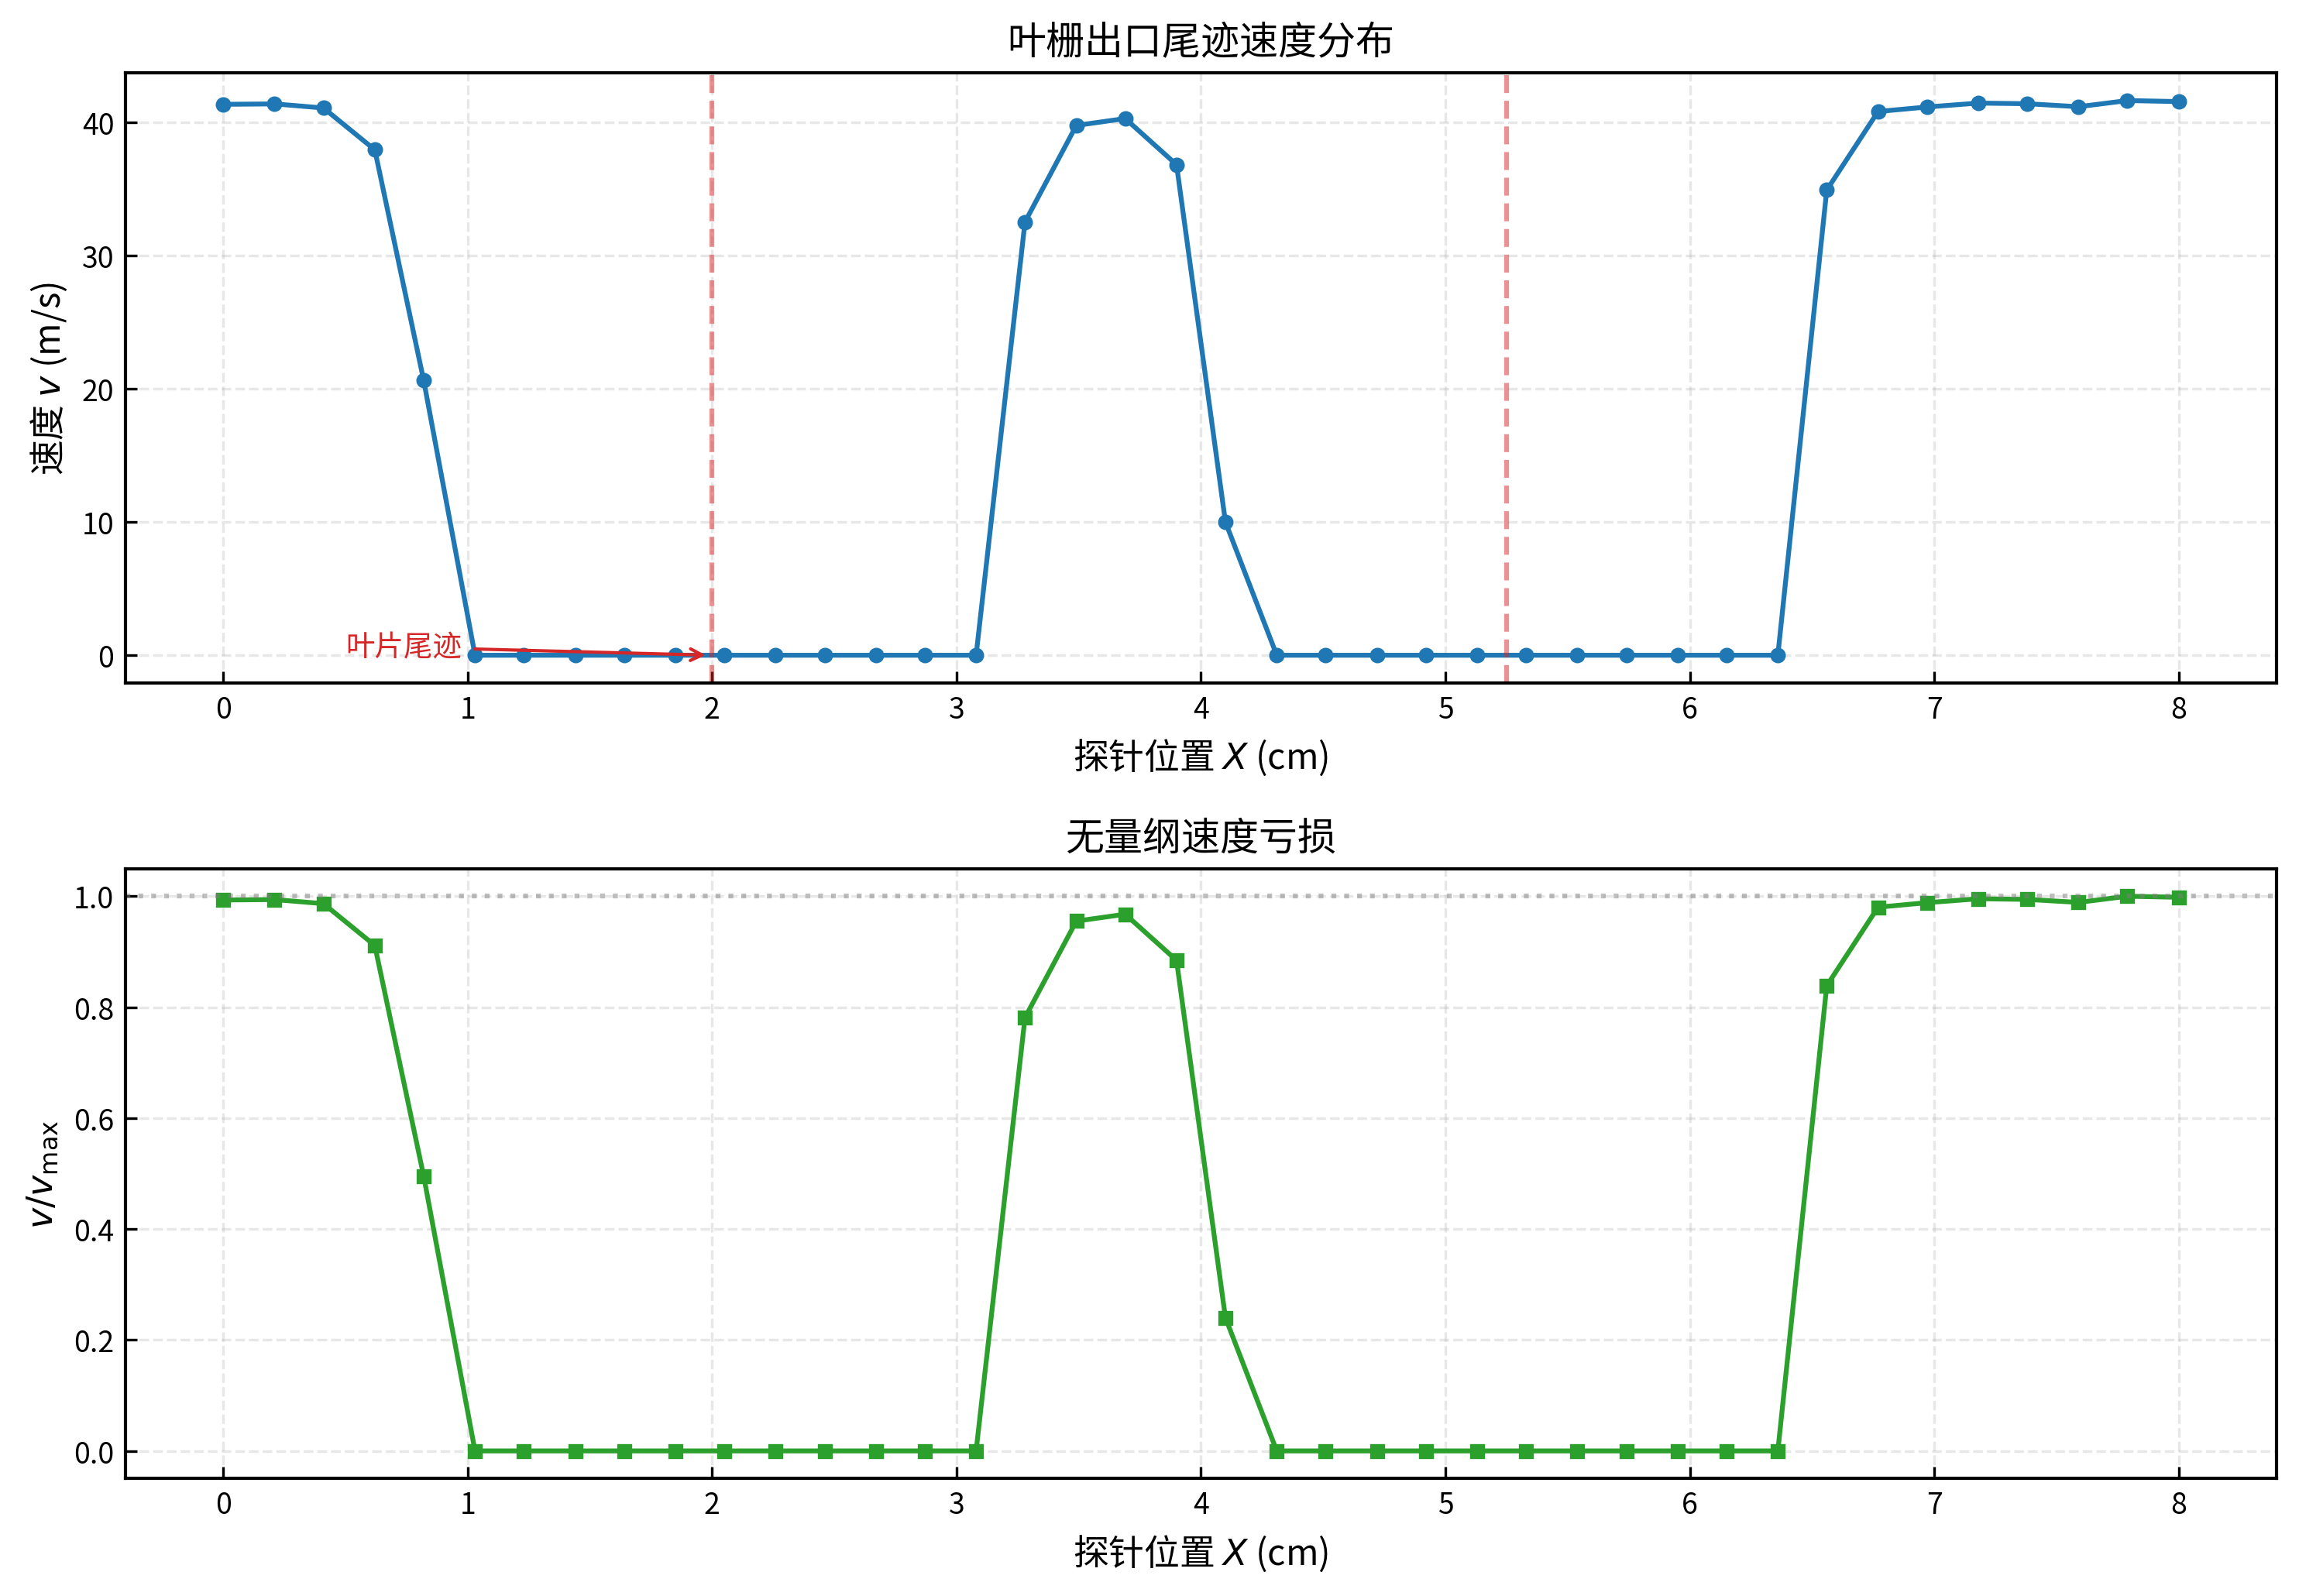
\includegraphics[width=0.85\textwidth]{figures/exp6_wake_velocity.png}
    \caption{叶栅出口尾迹速度分布（沿栅距方向扫描）}
    \label{fig:wake}
\end{figure}

图~\ref{fig:wake} 展示了沿栅距方向的速度分布。可以看出：
\begin{enumerate}
    \item 速度分布在叶片尾缘对应的周向位置出现明显的亏损（尾迹），呈周期性的"峰值-谷值"交替分布。
    \item 尾迹中心的速度亏损幅度约为主流速度的 20\%-40\%，具体数值取决于测量截面与尾缘的距离。
    \item 尾迹半宽（速度亏损降至一半时的宽度）约为叶片尾缘厚度的 2-3 倍。
    \item 相邻尾迹的间距约等于栅距（32.5 mm），与叶片数一致。
    \item 两个尾迹之间的主流区速度分布相对均匀，为叶栅通道内的核心流动区。
\end{enumerate}

\subsubsection{尾迹损失机制——边界层理论解释}

尾迹损失是叶型损失的三大组成部分之一（另两部分为附面层摩擦损失和激波损失）。其物理过程可概括为：

\begin{enumerate}
    \item \textbf{附面层发展}：气流流经叶片吸力面和压力面时，壁面附近形成附面层。附面层内速度梯度产生黏性剪切应力，消耗流体动能。
    \item \textbf{尾缘脱体}：在叶片尾缘，吸力面和压力面的两股附面层汇合，从叶片表面脱体。由于尾缘厚度不为零，脱体后的流动存在一个有限宽度的速度亏损区。
    \item \textbf{尾迹掺混}：尾迹内的低速流体与主流高速流体之间发生强烈的湍流掺混（动量交换），产生雷诺应力，将主流动能耗散为热能（不可逆熵增），表现为总压损失。
    \item \textbf{尾迹扩散}：随下游距离增大，尾迹宽度逐渐增大（扩散），速度亏损幅度逐渐减小（恢复），最终尾迹与主流完全掺混，总压损失不再变化。
\end{enumerate}

\subsection{结论}

通过三孔探针周向扫描，成功测量了NACA-65叶栅出口截面的尾迹速度分布。实验清晰识别了叶片尾缘对应的周期性速度亏损区，尾迹间距等于栅距（32.5 mm），速度亏损幅度约 20\%-40\%。尾迹损失的物理机制符合黏性边界层脱体和湍流掺混理论，是叶轮机械叶型损失的重要组成部分。掌握尾迹测量和分析方法对叶栅气动设计和损失评估具有重要意义。
